\documentclass[12pt,a4paper]{report}
\usepackage[utf8]{inputenc}
\usepackage[italian]{babel}
\usepackage{graphicx}
\usepackage{geometry}
\geometry{a4paper, margin=2.5cm}
\usepackage{bookmark}
\usepackage{hyperref}
\usepackage{amsmath}
\usepackage{float}
\usepackage{setspace}
\onehalfspacing

\title{\Huge\bfseries Relazione di Progetto: \\ Sistema Multi-Agente di Raccolta ed Esplorazione}
\author{\textbf{Mattia Campanella} \\ \textbf{Matricola: 1000029793} \\[1em] A.A. 2025/2026}
\date{}

\begin{document}

\maketitle

\begin{abstract}
Questa relazione presenta l'analisi, la progettazione e l'implementazione di un sistema multi-agente che opera all'interno di un ambiente a griglia. Verranno approfondite le euristiche decisionali e i processi cognitivi che guidano il comportamento di tre diverse tipologie di agenti: Scout, Collector e Hybrid. Attraverso una serie di esperimenti su layout differenti, vengono valutate le prestazioni degli agenti in termini di efficienza di esplorazione spaziale, ottimizzazione della raccolta delle risorse e gestione dei trade-off tra le varie mansioni autonome. L'analisi comparativa finale evidenzia i vantaggi e i limiti delle architetture specializzate rispetto a quella ibrida.
\end{abstract}

\tableofcontents
\newpage

\chapter{Introduzione e Specifiche dell'Ambiente}
\section{Il Problema dell'Esplorazione e della Raccolta}
Il problema affrontato in questo progetto appartiene all'area dell'Intelligenza Artificiale Distribuita (DAI). Si richiede ad un gruppo di agenti autonomi di operare in sinergia per esplorare un ambiente incognito, localizzando e raccogliendo un insieme di risorse (oggetti) per poi depositarle all'interno di zone di consegna (magazzini o warehouses). 

Le sfide principali derivano dall'osservabilità parziale dell'ambiente. Gli agenti non possiedono la posizione degli oggetti e devono pertanto esplorare la mappa iterativamente attraverso le loro percezioni locali. Questo approccio costringe l'agente a prendere decisioni online piuttosto che affidarsi a una pianificazione offline.

\section{Caratteristiche dell'Ambiente a Griglia}
L'ambiente simulato è rappresentato tramite una griglia bidimensionale discreta. Ogni cella della griglia può assumere diversi stati: essere libera, occupata da un ostacolo non attraversabile (muri), contenere un oggetto da raccogliere, o un'area di interesse strategico (entrate o uscite dei magazzini). 

\subsection{Visibilità degli agenti}
Un aspetto fondamentale della simulazione è la visibilità limitata degli agenti. Al tempo $t=0$, il sistema offre la possibilità di configurare la conoscenza a priori degli agenti: è possibile caricare direttamente in memoria l'intero layout della mappa (come la disposizione dei muri e le aree calpestabili). In questo caso la struttura della mappa è già nota agli agenti; rimangono tuttavia nascoste le posizioni degli oggetti e degli altri agenti. Alternativamente, si può scegliere di avviare la simulazione con l'intera griglia sconosciuta ad ogni agente.

La percezione visiva è definita da un raggio di visibilità (\texttt{VIS\_RANGE}), che circoscrive l'area entro cui l'agente può identificare le caratteristiche delle celle e la presenza di risorse o altri agenti. 

Per modellare realisticamente l'occlusione causata dagli ostacoli ambientali, si utilizza l'algoritmo di rasterizzazione delle linee di Bresenham. Questo algoritmo permette di determinare la line-of-sight tra l'agente e le celle rientranti nel suo raggio teorico: se la linea immaginaria incrocia un muro, le celle successive risultano opache e inosservabili.

\subsection{Limiti Energetici e Inizializzazione}
L'autonomia operativa di ogni entità è limitata da un livello di batteria iniziale (\texttt{INIT\_BATTERY}). Ogni spostamento all'interno della griglia consuma un punto di energia. La limitatezza delle risorse energetiche impone la necessità di trovare euristiche di navigazione complete ed efficienti.

\chapter{Dinamiche di Gioco e Comunicazione Sinergica}
\section{Mappatura Mentale e Conoscenza Distribuita}
Un sistema multi-agente si distingue per l'assenza intrinseca di un controllore centralizzato. Ogni individuo mantiene all'interno della propria memoria una sua personale rappresentazione spaziale del mondo in continuo aggiornamento. 

L'architettura adottata in questo progetto impone inoltre agli agenti di comunicare fra di loro per aggiornare la loro conoscenza del mondo di gioco. 

\section{Il Meccanismo della Comunicazione}
La condivisione delle informazioni non è continua, ma dipendente dalla prossimità tra gli agenti. Viene definito un raggio di comunicazione (\texttt{COMM\_RANGE}): quando due agenti si trovano nelle rispettive aree di comunicazione — definite dalla distanza di Chebyshev (il massimo tra la differenza assoluta di righe e quella di colonne, equivalente al raggio di un quadrato attorno all'agente) — viene eseguita un'unione bidirezionale dei dati.

Durante la comunicazione, gli agenti fondono reciprocamente le seguenti informazioni:
\begin{itemize}
    \item \textbf{Topologia della Mappa:} La percorribilità e conformazione delle celle scoperte.
    \item \textbf{Risorse Individuate:} Le coordinate di oggetti o dei magazzini scoperti lungo l'esplorazione.
    \item \textbf{Status degli Oggetti:} Gli oggetti già raccolti vengono rimossi dalla lista condivisa, in modo che nessun agente possa indirizzare un altro verso un oggetto già preso.
\end{itemize}

\chapter{Euristiche e Processi Decisionali degli Agenti}
In questo capitolo vengono descritte le logiche decisionali e l'architettura di ciascun tipo di agente.

\section{BaseAgent: Le Fondamenta Condivise}
La classe \texttt{BaseAgent} definisce le funzionalità comuni a tutti gli agenti: la gestione della batteria, la percezione dell'ambiente e il modulo di comunicazione. Ogni sottoclasse eredita la capacità di aggiornare la propria mappa locale e di scambiare informazioni con gli agenti vicini. Le posizioni degli altri agenti vengono associate al tick di osservazione, così da mantenere sempre la stima più recente in caso di aggiornamenti in conflitto.

\section{ScoutAgent: Esplorazione Pura (Frontier-based Search)}
Lo \texttt{ScoutAgent} eredita le capacità di base e si specializza nell'esplorazione della mappa. Opera secondo la strategia \textit{Frontier-based Search}, in cui l'agente si dirige sempre verso i bordi delle aree già esplorate per scoprire nuove celle:
\begin{enumerate}
    \item \textbf{Identificazione delle Frontiere:} Tramite una \textit{Breadth-First Search} (BFS) — algoritmo che visita le celle in ordine di distanza crescente, garantendo il percorso più breve in grafi non pesati — l'agente individua le celle percorribili note che confinano con almeno una cella ancora inesplorata (la ``frontiera'').
    \item \textbf{Euristica di Dispersione:} Dirigersi sempre alla frontiera più vicina porterebbe più agenti nella stessa area. Per evitarlo, lo Scout calcola uno score per ogni frontiera con la formula: $\texttt{score} = d_{BFS} - d_{agenti}$, dove $d_{BFS}$ è la distanza BFS dalla posizione corrente alla frontiera e $d_{agenti}$ è la distanza di Manhattan minima tra la frontiera e qualunque altro agente noto. Una frontiera vicina ad altri agenti ottiene uno score alto e viene quindi evitata, favorendo una copertura distribuita della mappa.
\end{enumerate}

\section{CollectorAgent: La Raccolta Orientata agli Obiettivi (FSM)}
Il processo decisionale del CollectorAgent è specializzato alla raccolta di oggetti. Il suo comportamento è definito da una \textit{Finite State Machine} (FSM): un modello in cui l'agente si trova sempre in uno stato preciso e transisce a un nuovo stato al verificarsi di condizioni specifiche. La FSM ha quattro stati:
\begin{enumerate}
    \item \textbf{EXPLORING:} Si dirige verso la frontiera più vicina tramite BFS, senza l'euristica di dispersione degli Scout. Se individua (visivamente o via comunicazione) la posizione di un magazzino e di almeno un oggetto abbandonato, transisce allo stato \textit{TARGETING}.
    \item \textbf{TARGETING:} Il collector smette di esplorare e si dirige verso l'oggetto più vicino tramite BFS. La distanza di Manhattan — somma delle differenze assolute di riga e colonna — viene usata per scegliere quale oggetto puntare tra quelli noti. Se durante il tragitto scopre che l'oggetto è già stato raccolto da un altro agente, ricalcola il target scegliendo quello successivo oppure tornando all'esplorazione.
    \item \textbf{DELIVERING:} Quando l'agente raggiunge la posizione dell'oggetto, lo raccoglie e si dirige verso la cella di ingresso (\texttt{ENTRANCE}) del magazzino più vicino.
    \item \textbf{EXITING:} Dopo aver consegnato l'oggetto, l'agente si sposta verso la cella di uscita (\texttt{EXIT}) del magazzino per liberare l'ingresso e non bloccare altri agenti in arrivo. Raggiunta l'uscita, decide se tornare a \textit{EXPLORING} oppure a \textit{TARGETING} se esistono ancora oggetti noti da raccogliere.
\end{enumerate}

\newpage

\section{HybridAgent: Adattività all' ambiente}
HybridAgent combina le strategie dei due agenti specializzati:
\begin{itemize}
    \item \textbf{Esplorazione Avanzata:} All'interno dello stato \textit{EXPLORING}, utilizza la stessa euristica di dispersione dello ScoutAgent, privilegiando le frontiere lontane dagli altri agenti.
    \item \textbf{Transizione Ritardata alla Raccolta:} A differenza del CollectorAgent, che passa a raccogliere non appena individua un oggetto e un magazzino, l'HybridAgent aspetta che il numero totale di oggetti scoperti o già consegnati raggiunga una soglia (9 nel codice attuale) prima di passare a \textit{TARGETING}. Questo prolunga la fase di esplorazione collettiva, aumentando la percentuale di mappa coperta prima di iniziare le consegne.
\end{itemize}

\chapter{Analisi delle Performance e Risultati}
Diverse configurazioni di agenti sono state testate sui due layout forniti; qui vengono presentati i risultati ottenuti. Le configurazioni testate riguardano la conoscenza pregressa del layout della mappa degli agenti, la presenza di agenti hybrid, e la quantità di questi ultimi

\section{Comportamento su Layout A}

I due grafici mostrano rispettivamente il numero cumulativo di oggetti consegnati e la batteria media consumata nel tempo. Il caso migliore è quello di un singolo HybridAgent, 2 Scout e 2 Collector con la mappa già nota: riescono a consegnare tutti gli oggetti tra i primi, consumando poca batteria. Il caso peggiore è invece quello di 5 HybridAgent senza mappa, che impiegano più tempo a completare la consegna e consumano molta più energia. In generale, dare la mappa agli agenti porta un vantaggio concreto: non dover esplorare la struttura della griglia da zero riduce gli spostamenti inutili e permette di raggiungere gli oggetti e i magazzini più velocemente. L'effetto è particolarmente evidente confrontando 3 Scouts e 2 Collector con e senza mappa: la versione con mappa consuma circa il 25\% di batteria in meno a parità di oggetti consegnati.

\begin{figure}[H]
    \centering
    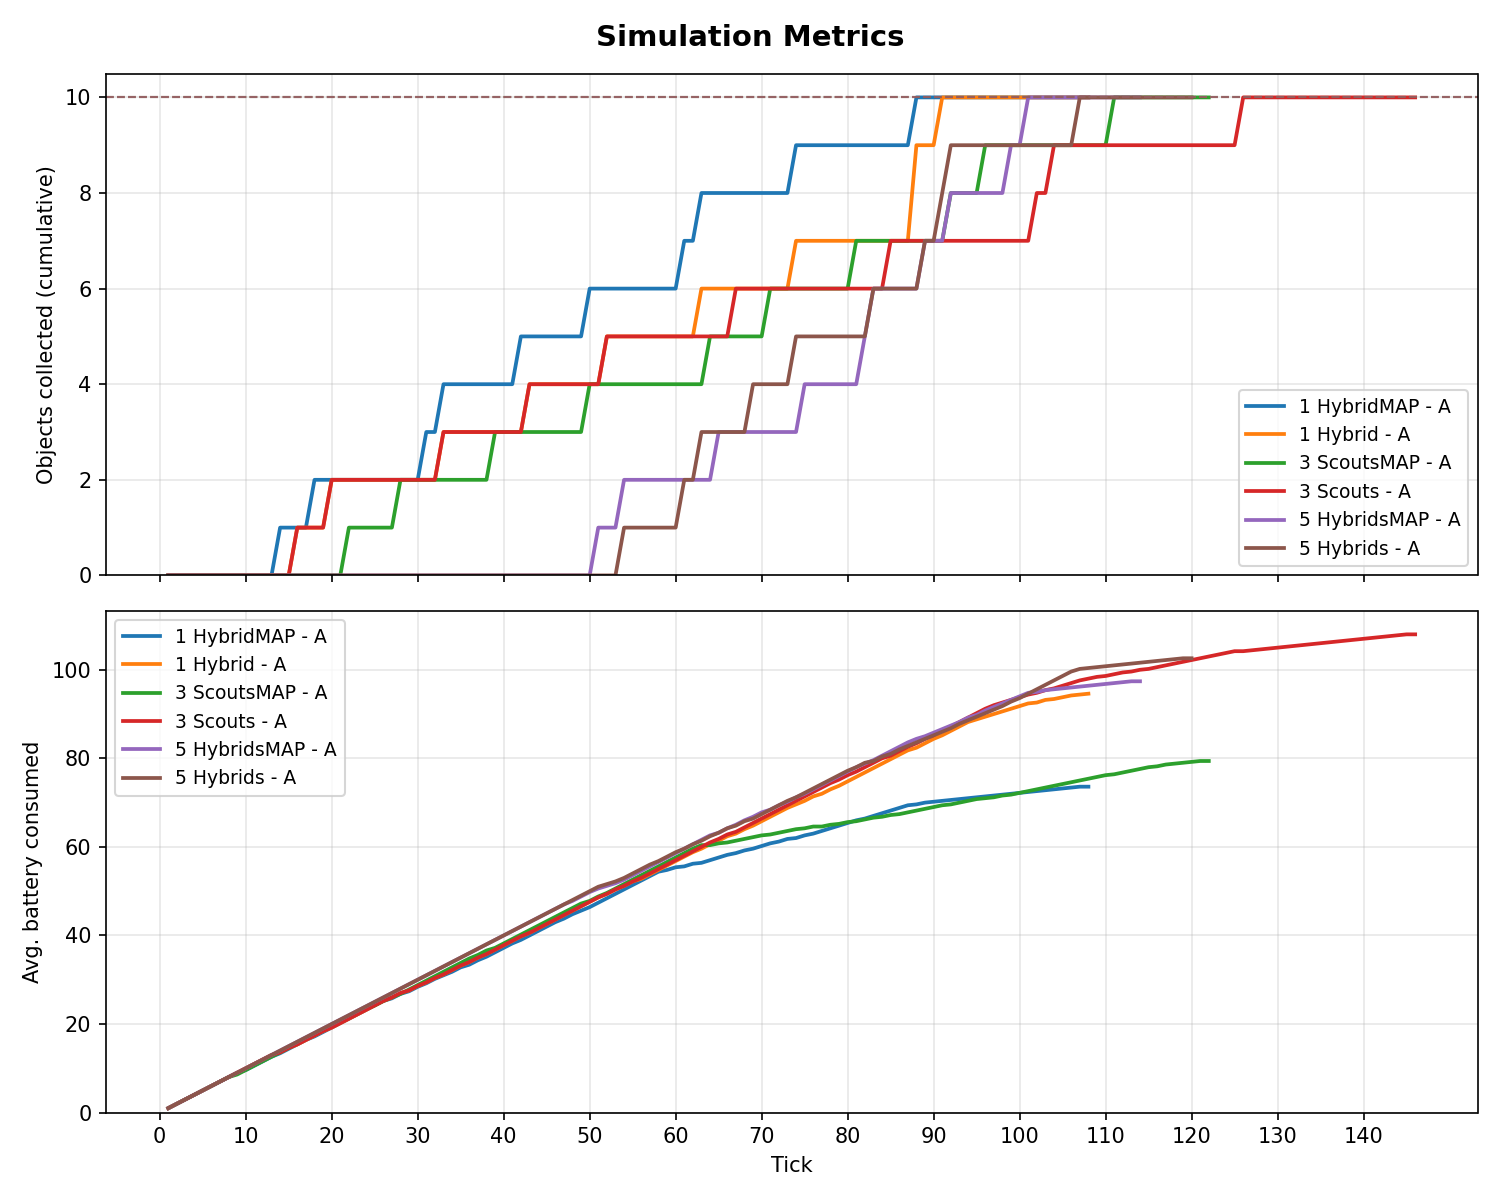
\includegraphics[width=0.9\textwidth]{img/comparisonA.png}
    \caption{Confronto tra configurazioni su Layout A: oggetti consegnati cumulativi e batteria media consumata nel tempo.}
    \label{fig:comparisonA}
\end{figure}

\section{Comportamento su Layout B (Geometria complessa)}

Anche qui i due grafici mostrano oggetti consegnati e batteria consumata nel tempo. Il caso migliore è 5 Hybrid con mappa: completano la consegna di tutti gli oggetti intorno al tick 90, con un consumo di batteria contenuto. Il caso peggiore è invece 3 Scout e 2 Collector senza mappa: non riescono a consegnare tutti gli oggetti prima delle altre simulazioni nonostante inizino le consegne per primi, mentre il caso 5 Hybrid senza mappa ha il consumo di batteria medio maggiore. In questo layout il vantaggio della mappa è molto più marcato rispetto al Layout A: probabilmente la struttura labirintica rende la navigazione senza mappa particolarmente costosa. Inoltre è interessante notare come strategie che potrebbero sembrare più efficienti in teoria, non possono esserlo in tutti i contesti.

\begin{figure}[H]
    \centering
    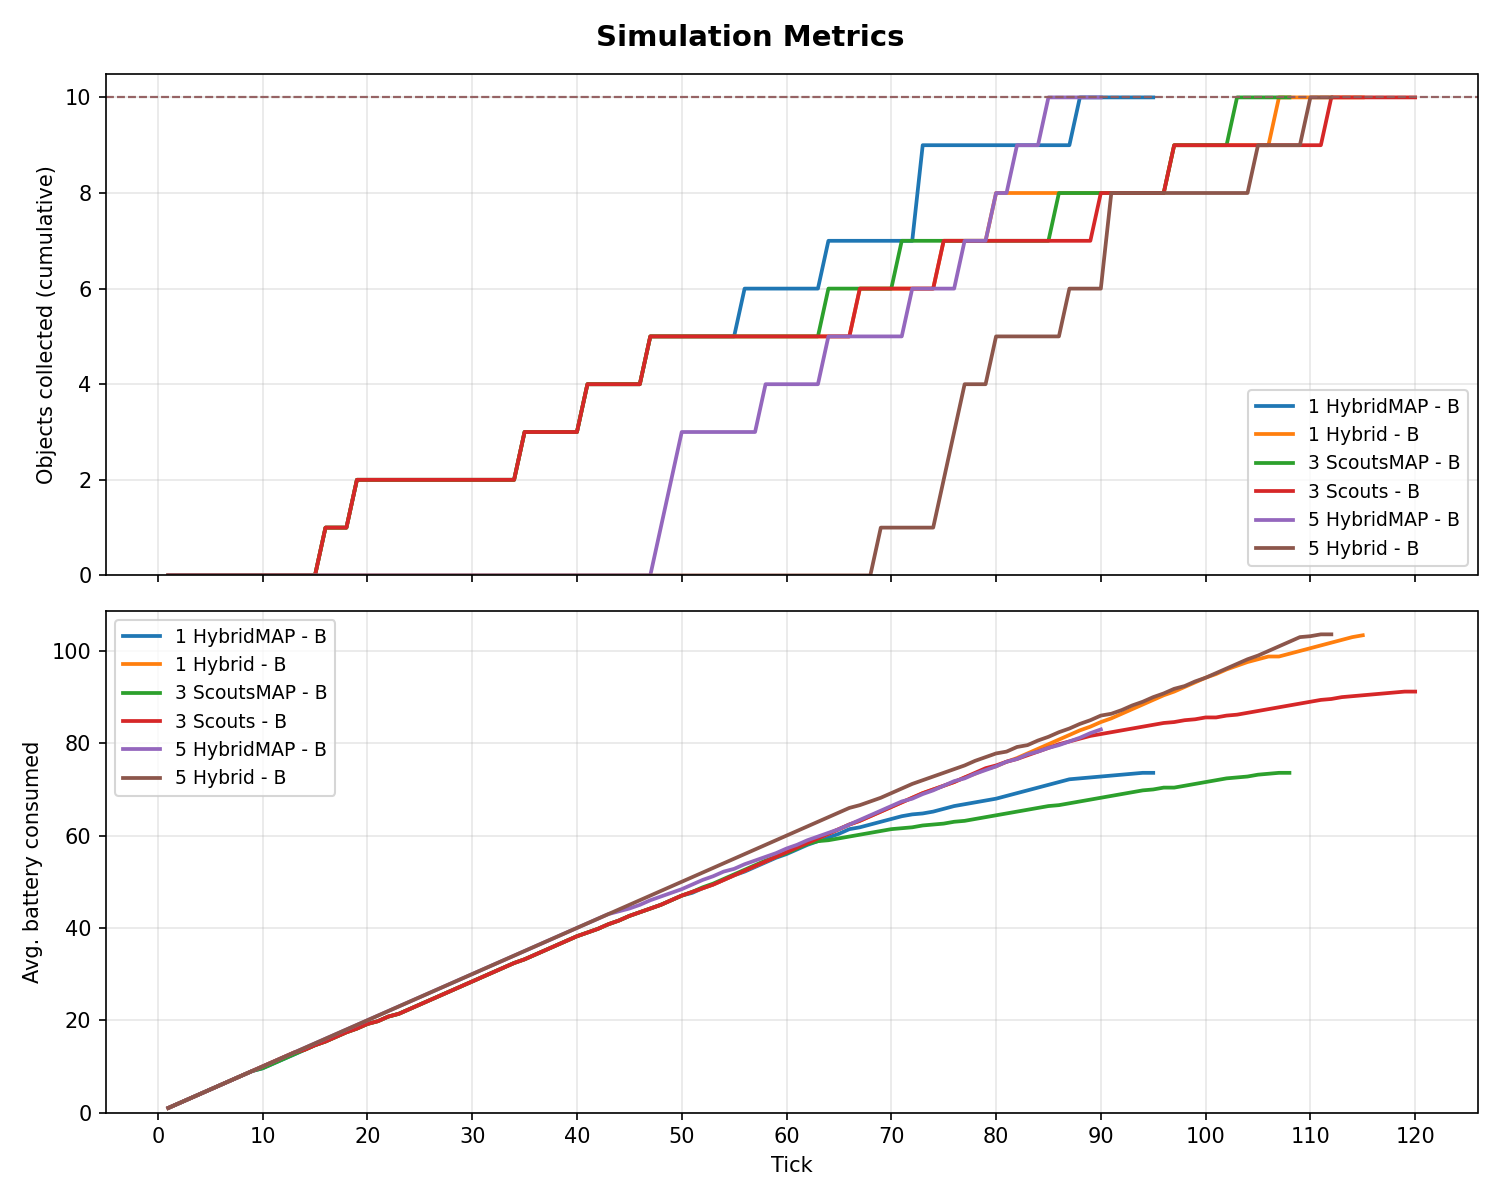
\includegraphics[width=0.9\textwidth]{img/comparisonB.png}
    \caption{Confronto tra configurazioni su Layout B: oggetti consegnati cumulativi e batteria media consumata nel tempo.}
    \label{fig:comparisonB}
\end{figure}


\chapter{Conclusioni}
L'architettura proposta ha messo in evidenza vantaggi e limiti delle diverse strategie adottate nel sistema multi-agente. I risultati mostrano che una divisione rigida tra scout e collector funziona bene in mappe semplici, dove la comunicazione tra agenti resta frequente; in ambienti labirintici, invece, questa dipendenza dalla comunicazione riduce l'efficacia complessiva.

L'approccio hybrid, basato su una FSM con fase iniziale di esplorazione estesa e raccolta ritardata, risulta più robusto nei contesti complessi. Questa soluzione riduce i movimenti non necessari, migliora l'uso della batteria e aumenta la probabilità di completare la consegna degli oggetti entro un numero minore di tick.

\end{document}
